% 12-two-exhibit-types
\begin{frame}[c]{Two exhibit types}
\begin{columns}[T,onlytextwidth]
  \begin{column}{0.48\textwidth}
    \centering
    \begin{tikzpicture}
      \node[inner sep=0,outer sep=0] (artwork) {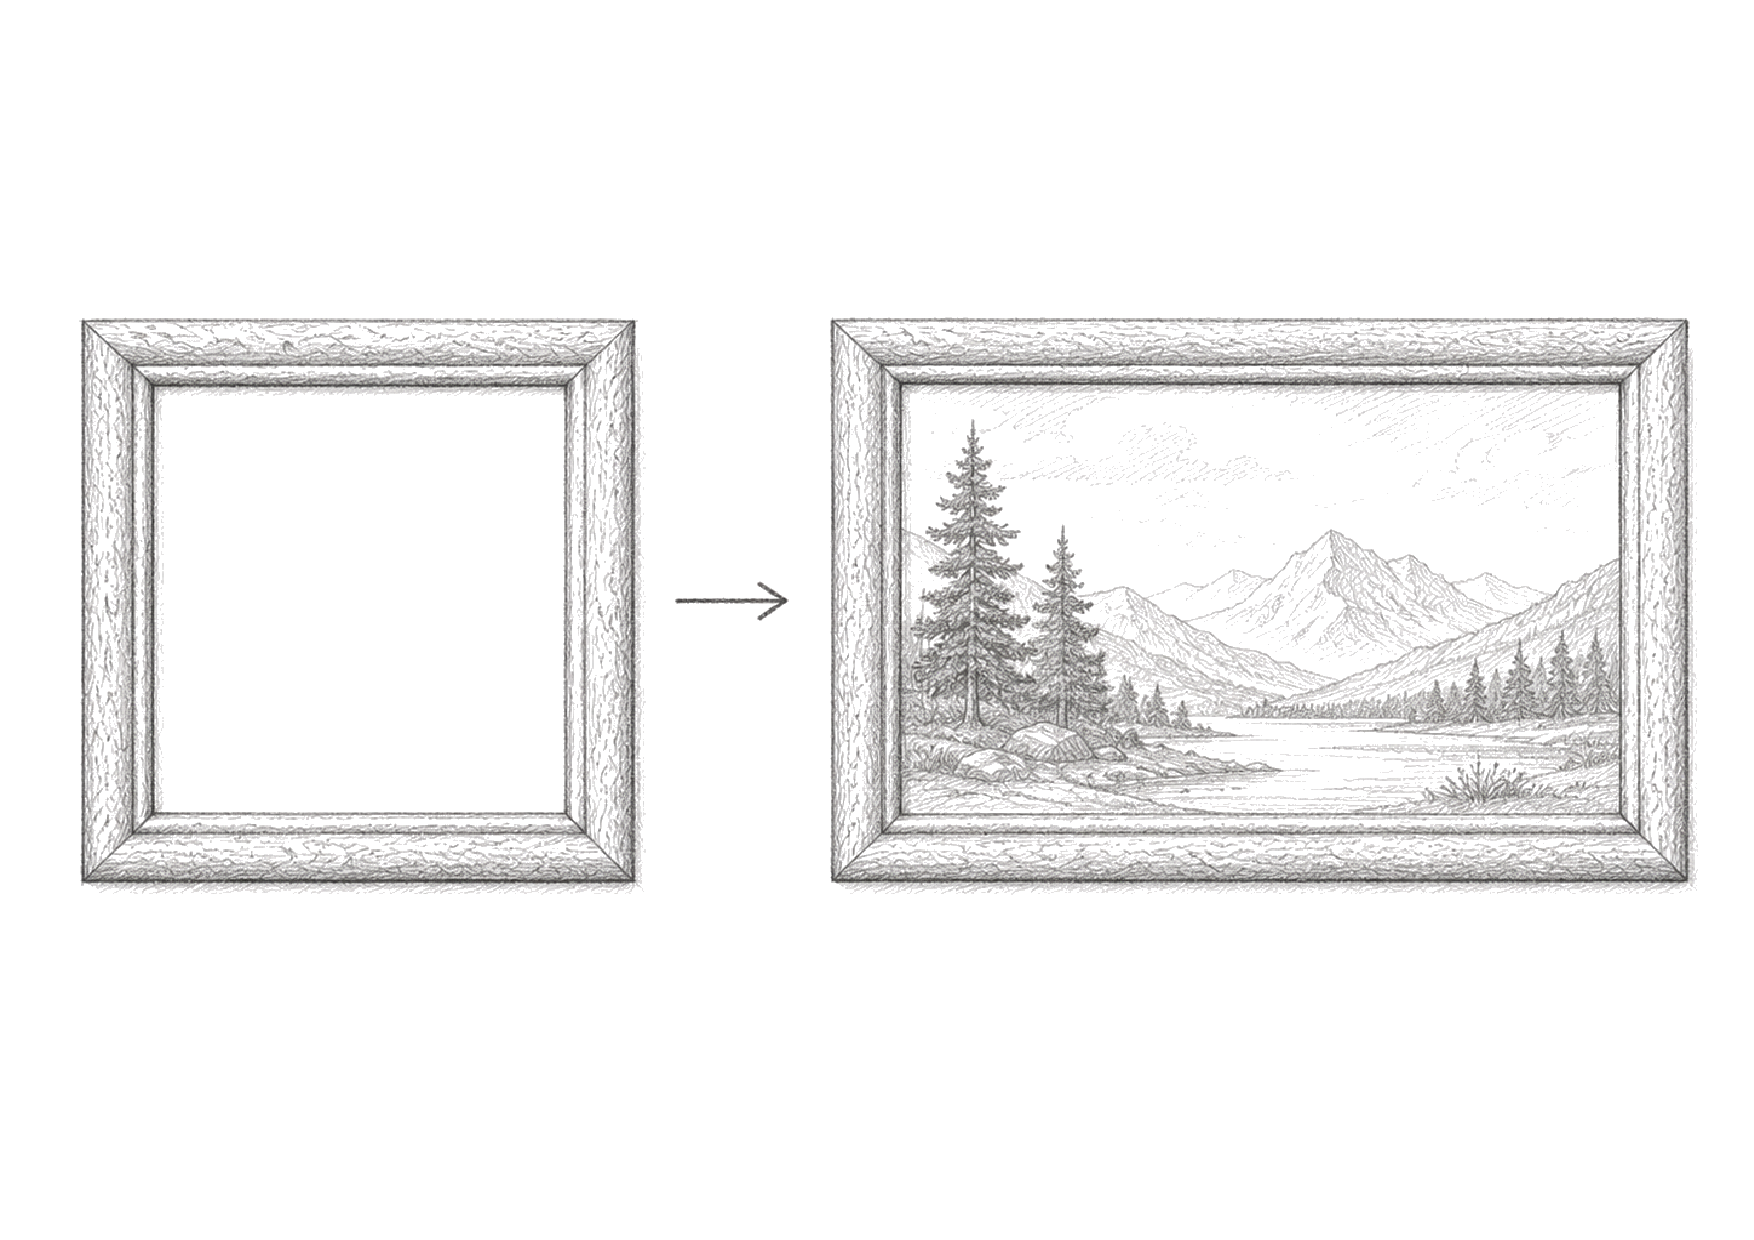
\includegraphics[height=3.35cm,keepaspectratio]{../Report/Figures/ch04-03-concept-2d-frame.pdf}};
      \node[anchor=south east,inner sep=1pt,text=black!65,font=\fontsize{4}{5}\selectfont]
        at ([xshift=-1pt,yshift=1pt]artwork.south east) {[GPT]};
    \end{tikzpicture}

    \vspace{0.10cm}
    \textcolor{unired}{\large\bfseries IMAGES \& VIDEOS}

    \vspace{0.08cm}
    \small
    Frames adapt to the media. Videos start at the matching segment.
  \end{column}
  \begin{column}{0.48\textwidth}
    \centering
    \begin{tikzpicture}
      \node[inner sep=0,outer sep=0] (artwork) {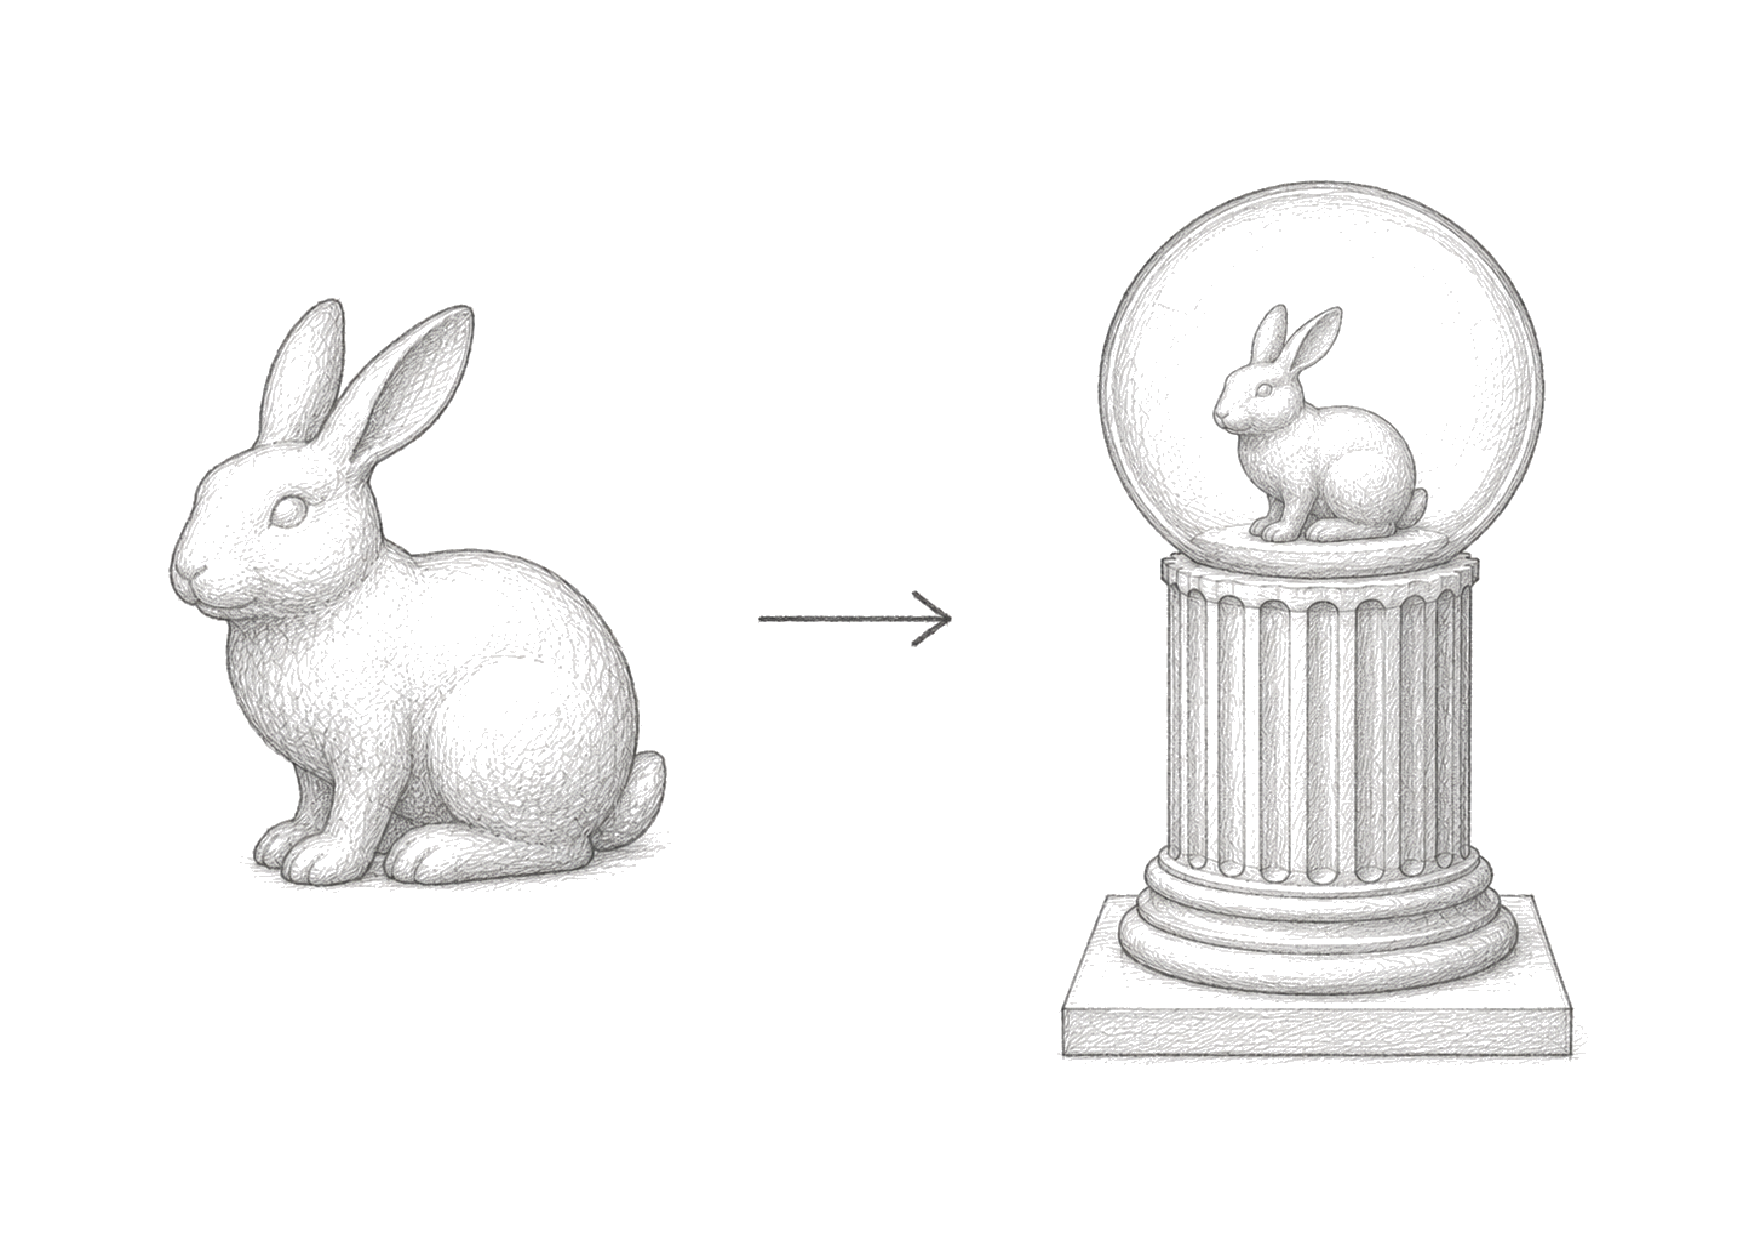
\includegraphics[height=3.35cm,keepaspectratio]{../Report/Figures/ch04-04-concept-3d-display.pdf}};
      \node[anchor=south east,inner sep=1pt,text=black!65,font=\fontsize{4}{5}\selectfont]
        at ([xshift=-1pt,yshift=1pt]artwork.south east) {[GPT]};
    \end{tikzpicture}

    \vspace{0.10cm}
    \textcolor{unired}{\large\bfseries 3D MODELS}

    \vspace{0.08cm}
    \small
    A fitted display. Inspection from every side.
  \end{column}
\end{columns}
\end{frame}
